Given that, the CDF of the given random variable is
$$
F_X(x)=\begin{cases}
			x/2, & 0<x<\frac{1}{2}\\
            x, & \frac{1}{2}\leq x\leq 1
		 \end{cases}
$$
% \begin{figure}[h]
%     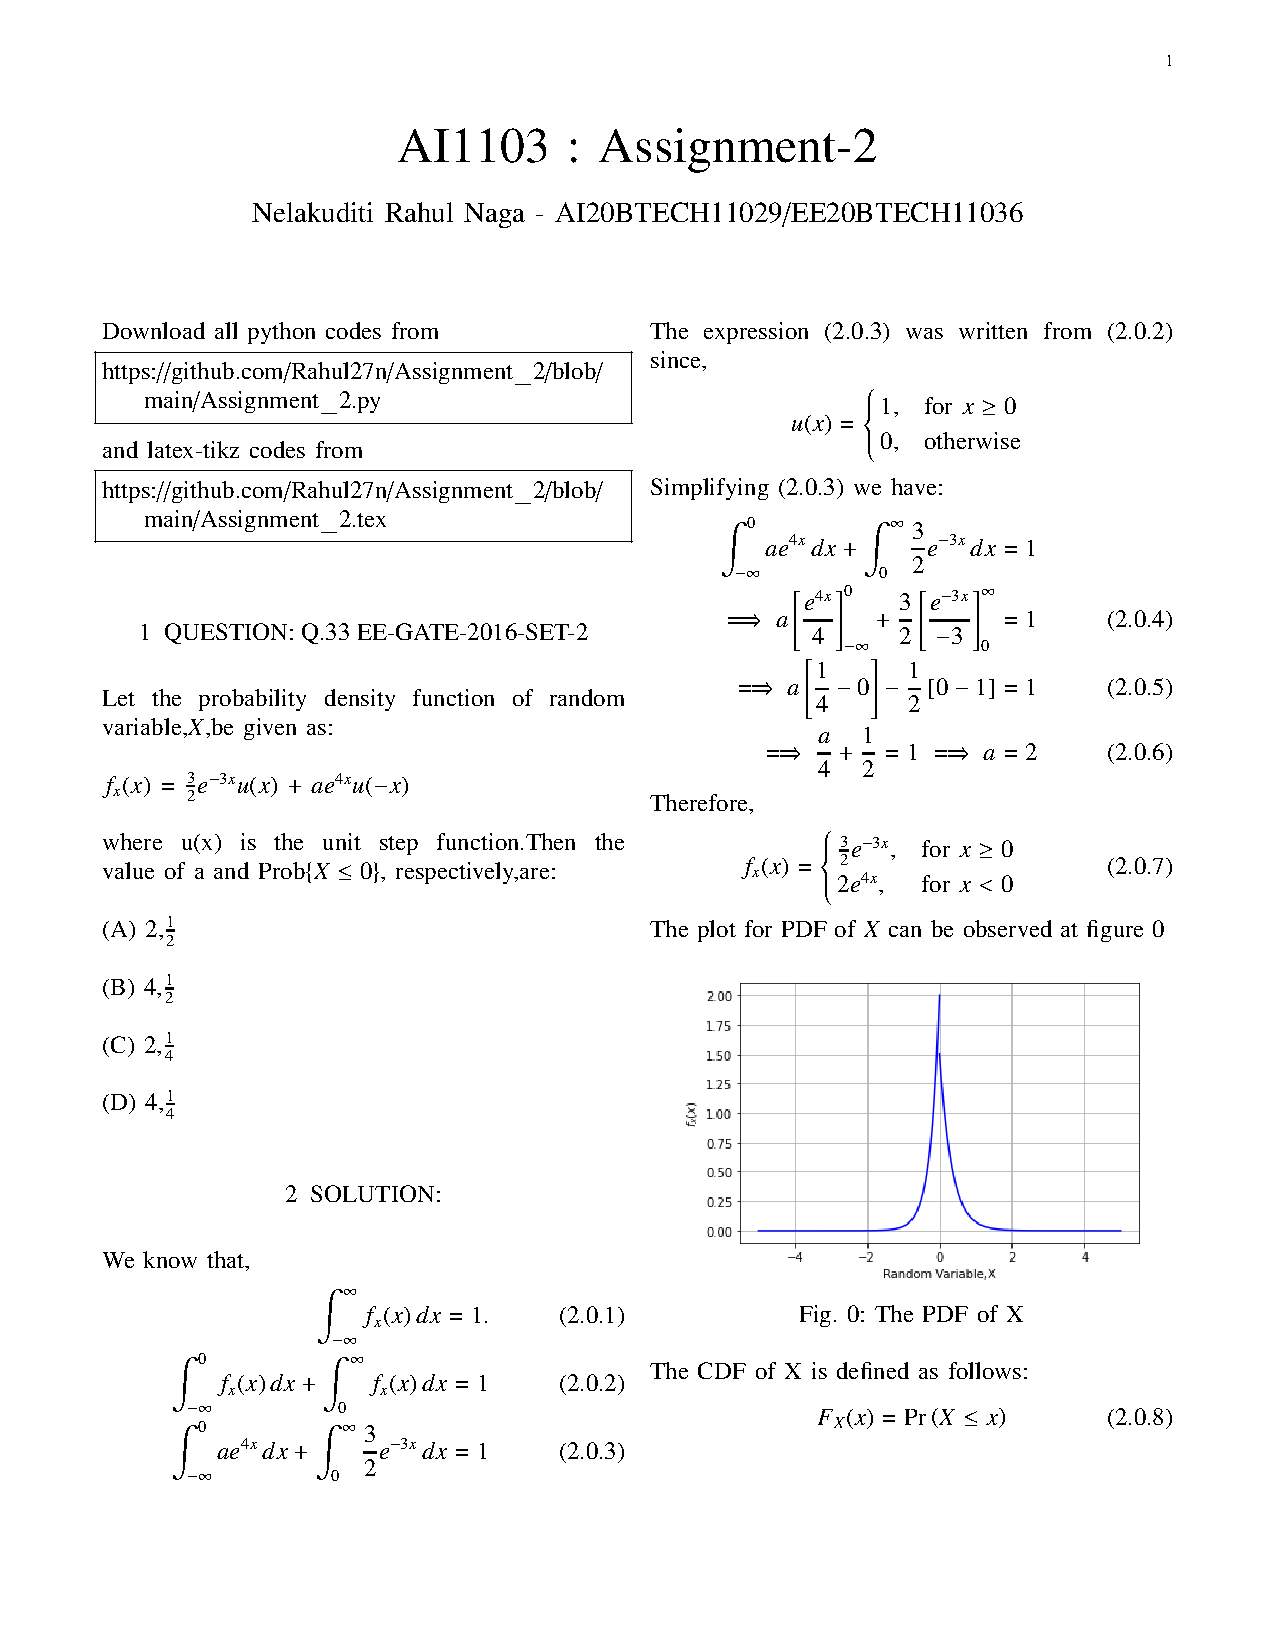
\includegraphics[width = 8cm]{images/Assignment_2.png}
% \end{figure}
that means probability of the random variable being $m$ is
\begin{align}
\Pr(X = m) =F_X(m) -  \lim_{t \to m^-}F_X(t)
\end{align}
Hence the probability value at $ X =\frac{1}{2}$ is
\begin{align}
    \Pr(X = 1/2) &= F_X\brak{\dfrac{1}{2}} -\lim_{t \to \frac{1}{2}^-}F_X(t)\\
    &= \frac{1}{2} - \lim_{x \to \frac{1}{2}^-} \frac{x}{2}\\
    &= \frac{1}{2} - \frac{1}{4}\\
    &= \frac{1}{4} = 0.25
\end{align}
